%------------------------------------------------------------
%	CAPITULO I
%------------------------------------------------------------

\chapter{Modelo Gavilán}
\label{capII}


%------------------------------------------------------------
%	Competencia de Manejo de Información (CMI)
%------------------------------------------------------------

\section{Competencia de Manejo de Información (CMI)}
\label{secCMICap2}

La Internet es la red de comunicación más grande del mundo, en la que se transmiten millones de datos y se consultan grandes cantidades de información al día. A partir del gran crecimiento de información que se encuentra en la web, se vuelve complicado identificar información útil, relevante e importante para la investigación de algún tema particular, ya que existe gran variedad de autores y fuentes que tratan un mismo tema.

A partir de la dificultad de encontrar información en una red tan grande como la Internet, se desarrollaron algunas estrategias para realizar investigaciones de mayor calidad, enfocada principalmente a estudiantes.

% REFERENCIA
López (2007) señala que la competencia de manejo de información (CMI) es un conjunto de habilidades, conocimientos y actitudes que el estudiante necesita para poder identificar puntualmente qué es lo que requiere saber sobre un tema, buscar la información de la mejor forma, señalar si la información responde a sus necesidades y convertirla en conocimiento útil para aplicarla en diferentes contextos.

La CMI fomenta y desarrolla las habilidades necesarias para obtener la capacidad de formular preguntas específicas que concreten la información que se requiere obtener, la elaboración de una estrategia que permita sintetizar y analizar la información de las preguntas formuladas, identificar y encontrar las fuentes más útiles y confiables, encontrar en su contenido la información buscada, evaluar la calidad la información tomando como base las necesidades a resolver en la investigación, clasificar la información para facilitar la síntesis, analizar y sintetizar la información en un formato útil y claro.

% REFERENCIA
De acuerdo con López (2007), una competencia es la combinación de dos factores importantes que son las capacidades y las actitudes (ver Figura \ref{fig:21}). Por un lado, la capacidad se compone de conocimientos y habilidades, que es todo aquello que se sabe y se conoce junto con todo aquello de lo que se puede hacer de forma correcta. Por otro lado, la actitud se refiere a las disposiciones. Es decir, que para poder lograr una competencia, se debe contar con la capacidad, que involucra saber, conocer, hacer, y también se debe contar con actitud, la buena disposición a lograr un objetivo.

\begin{figure}[H]
% \begin{figure}
  \centering
  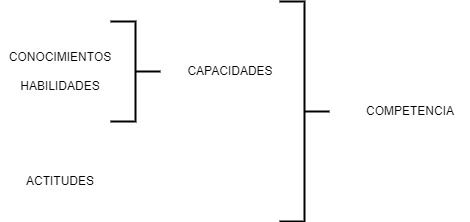
\includegraphics[width=0.70\textwidth]{Cap2/Figuras/CMI.jpg}
  \caption{Elementos constitutivos de capacidades y competencia. López (2007)}
  \label{fig:21}
\end{figure}

La abrumadora cantidad de información en la web y el desarrollo de la competencia de manejo de información, dio paso a la creación de metodologías que orientan el proceso de investigación de información. A estas se le conocen como metodologías para el desarrollo de la CMI.

%------------------------------------------------------------
%	Metodologías para el desarrollo de la CMI
%------------------------------------------------------------

\section{Metodologías para el desarrollo de la CMI}
\label{secMetodologiasCap2}

El proceso para desarrollar las habilidades de identificar y analizar las decisiones involucradas en la búsqueda de información, requiere de un proceso en el que se definen los pasos a seguir para adquirir buenos hábitos de investigación y convertirlos en una habilidad en la práctica.

A partir de la necesidad de contar con un mecanismo o una estrategia para adquirir las habilidades involucradas en la CMI, nacen diferentes metodologías que impulsan el desarrollo de la CMI. 

Estas metodologías consideran las propiedades base de la CMI, tales como realizar un proceso de búsqueda, análisis, organización y síntesis de la información encontrada en fuentes como libros, blog, páginas web, revistas, entre otros. Por otro lado, las metodologías también deben promover que los estudiantes utilicen  los conocimientos adquiridos.

% REFERENCIAS
Actualmente, existen diferentes metodologías que definen un conjunto de pasos para desarrollar la CMI. González y Sánchez (2007) señalan que algunas de las metodologías existentes son las siguientes:

\begin{itemize}
  \item La metodología de la Asociación de Bibliotecas Escolares de Ontario, Canadá.
  \item La metodología \textit{Big 6}, creada por Eisenberg y Berkowitz.
  \item La metodología \textit{Ciclo de Investigación} creada por Jaime Mckenzie.
  \item La metodología \textit{Modelo de Proceso para Búsqueda de Información (ISP)}, creada por Carol Kuhlthau.
  \item El \textit{Modelo de Irving para Competencias para el Manejo de la Información}, creado en Reino Unido.
  \item El \textit{Modelo de Stripling y Pitts del Proceso de Investigación}, creado en Estados Unidos.
  \item El \textit{Modelo Gavilán}, de la Fundación Gabriel Piedrahita Uribe, creada en Colombia.
\end{itemize}

Cada una de las metodologías tiene un comportamiento diferente pero todas pretenden lograr el mismo objetivo, desarrollar la CMI.
 
La mayor parte de estos modelos dividen su estrategia de búsqueda de información de entre cuatro pasos a 16 pasos, los cuales se agrupan en 4 etapas principales: búsqueda de fuentes, análisis y evaluación, interpretación, y síntesis de la información.

%------------------------------------------------------------
%	Pasos del Modelo Gavilán
%------------------------------------------------------------

\section{Pasos del Modelo Gavilán}
\label{secPasosCap2}

% REFERENCIA
González y Sánchez (2007) señalan que el Modelo Gavilán es un modelo que surge en Colombia por la Fundación Gabriel Piedrahita Uribe. Este modelo fue dividido en cuatro etapas que conforman el proceso de investigación de información, basado en los objetivos de la CMI.

Los cuatro pasos que conforman el Modelo Gavilán son: 1) definir el problema de investigación, 2) buscar y evaluar información, 3) análisis de la información y 4) sintetizar la información. Estos pasos se siguen como en la Figura \ref{fig:22}.

\begin{figure}[H]
% \begin{figure}
  \centering
  \includegraphics[width=0.70\textwidth]{Cap2/Figuras/Modelo Gavilán.jpg}
  \caption{Pasos fundamentales del Modelo Gavilán. González y Sánchez (2007)}
  \label{fig:22}
\end{figure}

A su vez, cada paso definido en el Modelo Gavilán, contiene una serie de subpasos, en los que se divide específicamente la acción que se debe realizar al momento de realizar una investigación.

%------------------------------------------------------------
%	Definición del problema de investigación
%------------------------------------------------------------

\subsection{Definición del problema de investigación}
\label{secPaso1Cap2}

La etapa de definición del problema de la investigación tiene como objetivo desarrollar las habilidades necesarias para delimitar la búsqueda de información de un tema, así como desarrollar estrategias para plantear un problema de información y establecer un límite para conocer con cierta exactitud el rubro del tema que se quiere conocer.

Para lograrlo, es importante definir la necesidad de información en un contexto o situación determinada, que enfoque el comienzo de la investigación en forma de una \textit{pregunta inicial}. Una vez definido qué es lo que se necesita investigar, se recurre a la identificación de temas centrales que abarquen la información que sea útil a la investigación, tales como conceptos, definiciones y descripciones relevantes del tema en el que se centra la información.

Los aspectos anteriores a desarrollar se dividen en subpasos que conforman el primer paso del Modelo Gavilán. Este se compone de los siguientes subpasos:

\begin{itemize}
  \item [1a.] Plantear una pregunta inicial
  \item [1b.] Analizar la pregunta inicial
  \item [1c.] Construir un plan de investigación
  \item [1d.] Formular preguntas secundarias
  \item [1e.] Evaluar el paso 1
\end{itemize}

Estos subpasos se siguen como en la Figura \ref{fig:23}.

\begin{figure}[H]
% \begin{figure}
  \centering
  \includegraphics[width=0.70\textwidth]{Cap2/Figuras/Definición del problema.jpg}
  \caption{Definición del problema de investigación. González (2007)}
  \label{fig:23}
\end{figure}

%------------------------------------------------------------
%	Subpaso 1a: Plantear una pregunta inicial
%------------------------------------------------------------

\subsubsection{Subpaso 1a: Plantear una pregunta inicial}
\label{secPaso1aCap2}

El objetivo de este subpaso es que los estudiantes adquieran la habilidad de iniciar una investigación, a partir de la formulación de preguntas iniciales para plantear problemas de información. Con este subpaso, se busca que el estudiante comprenda la utilidad de comenzar la exploración de un tema, con base en preguntas para delimitar un tema nuevo que probablemente es desconocido para el estudiante. Asimismo, se tiene como objetivo identificar una pregunta inicial adecuada, que es aquella que mejor delimita el tema de la investigación.

Es importante mencionar que no todas las preguntas generadas de un tema son preguntas iniciales. Las preguntas iniciales adecuadas abarcan diferentes conceptos, características, subtemas o aspectos de un tema. Es decir, son preguntas cuya respuesta no es concreta, como la fecha de un acontecimiento histórico, el lugar de nacimiento de algún personaje, etc. Por el contrario, las preguntas iniciales son preguntas que pueden abarcar toda esta información de un tema, en donde está involucrada información que responde a las preguntas cómo, cuándo, dónde, etc. Este tipo de preguntas da la posibilidad a los estudiantes de realizar una tarea de reflexión sobre el tema de investigación, para dar contexto e identificar la importancia de obtener información diversa de un tema delimitado.

% REFERENCIA
González (2007) señala que una pregunta inicial surge a partir de un problema de información, y para que pueda formularse de forma adecuada, se deben cumplir dos características importantes que se presentan a continuación:

\begin{enumerate}
  \item Requerir información ya existente, que esté disponible en fuentes de información como páginas web, libros, revistas, enciclopedias, etc.
  \item Plantearse a partir de un contexto o situación real que despierte la curiosidad del estudiante, para analizar y aplicar los conocimientos que se adquieren durante la investigación.
\end{enumerate}

Por ejemplo, si un alumno quiere saber sobre matemáticas, se vuelve complejo investigar el tema de forma general, ya que la información que se puede encontrar sobre el tema es muy extensa. Sobre matemáticas podrían surgir preguntas como ¿qué son las matemáticas?, ¿qué es la álgebra?, ¿cómo se resuelven las derivadas?, ¿cómo se demuestra un teorema matemático?, e incluso preguntas como ¿las matemáticas se inventaron o se descubrieron? o ¿crees que eres malo para las matemáticas?

Para este ejemplo tomaremos como pregunta inicial la última propuesta, ¿crees que eres malo para las matemáticas?, la cual cumple con las dos características para formular una pregunta inicial adecuada mencionadas anteriormente. La respuesta a esta pregunta requiere de información que ya existe en diferentes fuentes de información, además de plantear si los conocimientos de esta pregunta pueden adaptarse a un contexto real.

%------------------------------------------------------------
%	Subpaso 1b: Analizar la pregunta inicial
%------------------------------------------------------------

\subsubsection{Subpaso 1b: Analizar la pregunta inicial}
\label{secPaso1bCap2}

Este subpaso consiste en desarrollar habilidades para examinar con detalle el límite de la pregunta inicial propuesta. En esta etapa se distinguen los distintos subtemas que pueden estar  englobados en la pregunta inicial, con el fin tener conocimiento sobre la información involucrada en la investigación. A su vez, se determina si el enfoque de la pregunta inicial es correcto de acuerdo con los propósitos de la investigación, es decir, que ésta pueda incluir todos aquellos puntos que son necesarios considerar y conocer como resultado de la investigación.

El análisis de una pregunta inicial permite crear un límite en la profundidad de la investigación de un tema y dar dirección al estudiante en forma de guía para delimitar un tema amplio, en detalles específicos, ya que por lo general, no es necesario conocer absolutamente todo el tema y los subtemas que se puedan derivar del mismo, sino que sólo es necesario incluir ciertos detalles en el proceso de investigación.

Los aspectos específicos de un tema, involucrados en la pregunta inicial, pueden considerarse como categorías, jerarquías o clases, dependiendo del contexto del tema, de tal manera que se forma una clasificación del contenido. Una estrategia para identificar esta clasificación de información, es manifestar, en forma oral o escrita, todo lo que se sabe sobre el tema de investigación en forma de hipótesis, que no necesariamente son verdaderas, tomando en cuenta aspectos que van desde lo más general hasta lo más particular y con ello tratar de responder a la pregunta inicial. El hecho de responder o dar una respuesta aproximada a la pregunta inicial aporta una pauta importante para identificar las clases, jerarquías o categorías del conocimiento que se quiere saber al final de la investigación.

Una segunda estrategia consiste en buscar información en Internet, libros, revistas o cualquier fuente de información, de forma rápida y no exhaustiva, es decir, una breve búsqueda sobre el tema sin involucrar detalles específicos, con el fin de generar una idea, de forma general, sobre el tema. Esta búsqueda permite producir ideas y conocimiento sobre aspectos sobresalientes del tema, que pueden representarse como posibles categorías. Con ello, se permite identificar aquellos temas que necesitan mayor profundidad y dar dirección a la información útil para responder la pregunta inicial.

Cabe mencionar que las dos estrategias anteriores son un apoyo para poder identificar las categorías y valorar sí la pregunta inicial es la más adecuada para comenzar la investigación. Ambas estrategias pueden usarse individualmente o como complemento una de la otra, para desarrollar de mejor manera el análisis de la pregunta inicial. En caso de que la pregunta inicial no contenga información útil para el conocimiento de la investigación final, será necesario considerar otra pregunta como pregunta inicial o reestructurar la formulación de la pregunta.

Retomando el ejemplo de la pregunta inicial seleccionada, ¿crees que eres malo para las matemáticas?, se presentan a continuación algunas hipótesis correspondientes a la primera estrategia e información de fuentes de información correspondientes a la segunda estrategia.

\begin{table}[H]
  \begin{center}
    \begin{tabular}{ | p{8cm} | p{8cm} | }
      \hline
      HIPÓTESIS (PRIMERA ESTRATEGIA) & FUENTES DE INFORMACIÓN (SEGUNDA ESTRATEGIA) \\ \hline
      \begin{itemize}
        \item Si me cuesta trabajo realizar cuentas, soy malo para las matemáticas.
        \item Si las matemáticas no son de mi interés, entonces soy malo en matemáticas.
        \item Si cualquier materia de matemáticas me aburre, entonces soy malo para matemáticas.
        \item Si no estudio alguna ingeniería, entonces no soy bueno en matemáticas.
        \item Si soy filósofo, entonces soy malo para las matemáticas.
      \end{itemize} & 
      \begin{itemize}
        \item Ruef (2020) señala que $"$El 'trauma matemático' se manifiesta como ansiedad o temor, un miedo debilitante a equivocarse.$"$
        \item Ruef (2020) señala que $"$los estudiantes que tienen éxito en las pruebas de datos matemáticos cronometrados, pueden creer que ser buenos en matemáticas$"$
        \item Sautoy (2015) señala que $"$muchos expertos advierten que el hablar de 'genes matemáticos' es una falacia, pues lo que se requiere para ser bueno en matemáticas es esforzarse$"$
      \end{itemize} \\ \hline
    \end{tabular}
    \caption{Ejemplo de estrategias del subpaso 1a del Modelo Gavilán.}
    \label{tab:t1}
  \end{center}
\end{table}

De la información presentada en la Tabla \ref{tab:t1}, podemos identificar aspectos para clasificar la información útil y necesaria para considerar en la investigación. Algunos aspectos de ellos pueden ser los siguientes:

\begin{itemize}
  \item Definición de trauma matemático.
  \item Aspectos a considerar para aprender matemáticas.
  \item Definición de genes matemáticos.
  \item Relación entre el trauma matemático y el desinterés o aburrimiento por las matemáticas.
  \item Escritores que son matemáticos.
\end{itemize}

%------------------------------------------------------------
%	Subpaso 1c: Construir un plan de investigación
%------------------------------------------------------------

\subsubsection{Subpaso 1c: Construir un plan de investigación}
\label{secPaso1cCap2}

Este paso consiste en desarrollar las habilidades para definir la organización y el orden en que se realizará la investigación. Una vez identificada una pregunta inicial adecuada, así como las distintas categorías que abarca, se planea el orden en que se comenzará a investigar cada una de las categorías, con el fin de dar el seguimiento más adecuado a la investigación en orden cronológico, jerárquico o por profundidad del tema.

La planeación de la forma de investigación permite obtener una guía durante el proceso de investigación, del cual se produce un objetivo más claro sobre la información que es adecuada y útil para la investigación final. En esta etapa también se considera un filtro de categorías que no aportan información relevante a la investigación, así como la identificación de las categorías que sí aportan información útil, para poder ordenarlas y dar seguimiento al orden en que se va a examinar cada una de las categorías identificadas en el subpaso 1b.

% REFERENCIA
González (2007), señala que una estrategia que se puede seguir para poder realizar un plan de investigación adecuado incluye los siguientes pasos:

\begin{itemize}
  \item Identificar las categorías que son más adecuadas para responder a la pregunta inicial. Por otra parte, omitir aquellas categorías que no aportan información útil para responder a la pregunta inicial, estas las podemos denominar como categorías secundarias.
  \item Determinar y decidir si las categorías encontradas en el paso anterior son suficientes para poder responder la pregunta inicial. En caso de que falten puntos por cubrir para responder la pregunta inicial, es necesario identificar cuáles son las categorías faltantes y agregarlas a las categorías actuales.
  \item Establecer el orden más adecuado para dar seguimiento a la investigación. El orden puede ser cronológico, por jerarquía, por profundidad, etc. Con ello se facilita la comprensión de la información para el mejor entendimiento del tema.
  \item Por cada una de las categorías ya ordenadas, identificar cuáles son los aspectos que son necesarios conocer y que aporten utilidad a la información final de la investigación.
\end{itemize}

Retomando el ejemplo anterior y las categorías antes identificadas. Siguiendo la estrategia mencionada anteriormente, el primer paso señala que es importante determinar cuáles categorías son importantes y desechar aquellas que no aportan contenido útil a la respuesta de la pregunta inicial. En este caso, no sería necesario conocer la definición de genes matemáticos, la relación entre el trauma matemático y el desinterés, así como saber información de filósofos que han sido matemáticos. Por lo que la lista se reduce como sigue:

\begin{itemize}
  \item Definición de trauma matemático.
  \item Aspectos a considerar para aprender matemáticas.
\end{itemize}

El segundo paso propone realizar un análisis para saber si las categorías son suficientes para responder a la pregunta inicial. En este caso, también puede ser de interés las causas del trauma matemático. Esta nueva categoría que se agrega queda como sigue.

\begin{itemize}
  \item Definición de trauma matemático.
  \item Aspectos a considerar para aprender matemáticas.
  \item Causas del trauma matemático.
\end{itemize}

El tercer punto menciona que es útil establecer un orden entre las categorías. En este caso, no es tan claro investigar las causas del trauma matemático sin antes saber qué es el trauma matemático, por lo que se debe investigar antes. Los aspectos a considerar para aprender y fortalecer la habilidad matemática se derivan de las causas, por lo que esta se puede investigar después. Estas observaciones modifican el orden de la lista de categorías como sigue.

\begin{itemize}
  \item Definición de trauma matemático.
  \item Causas del trauma matemático.
  \item Aspectos a considerar para aprender matemáticas.
\end{itemize}

Finalmente, se identifican aspectos específicos, en caso de haberlos, por cada una de las categorías:

\begin{itemize}
  \item Definición de trauma matemático.
    \begin{itemize}
      \item Quién define el concepto.
      \item Cuándo surge.
    \end{itemize}
  \item Causas del trauma matemático.
    \begin{itemize}
      \item A quiénes afecta.
      \item Cómo se manifiesta el trauma matemático.
    \end{itemize}
  \item Aspectos a considerar para aprender matemáticas.
    \begin{itemize}
      \item Tipo de ejercicios a considerar.
      \item Estrategias de práctica.
    \end{itemize}
\end{itemize}

%------------------------------------------------------------
%	Subpaso 1d: Formular preguntas secundarias
%------------------------------------------------------------

\subsubsection{Subpaso 1d: Formular preguntas secundarias}
\label{secPaso1dCap2}

Este paso consiste en identificar aquellos aspectos específicos de cada categoría que aporten información útil a la investigación final a partir de preguntas secundarias. Estas preguntas tienen el propósito de brindar información de aspectos específicos que son importantes mencionar en la investigación según lo propuesto en la construcción del plan de investigación.

Las preguntas secundarias tienen la característica de ser más concretas y apuntar a información más específica, ya que da respuesta a detalles precisos de algún tema, lo cual determina el contenido que apoya a responder la pregunta inicial en conjunto.

Para poder crear las preguntas secundarias, es necesario tomar los aspectos que son necesarios conocer en la investigación, mismos que fueron identificados en el paso 1c. Una vez que se tiene el conjunto de aspectos a conocer, se procede a convertir cada característica específica en una pregunta, de tal forma que la pregunta pueda darle una respuesta concreta, sin perder de vista que estas preguntas no deben ser muy sencillas ni muy complejas.

Tanto el plan de investigación como la creación de preguntas secundarias, puede ir creciendo conforme avanza la investigación, con el fin de retroalimentar la información con detalles faltantes o a forma de complemento, sin embargo, es recomendable que los aspectos importantes de la investigación, así como las preguntas secundarias, queden bien definidas durante la primera etapa de definición del problema, para que no exista confusión durante los siguientes pasos del Modelo Gavilán.

Para este ejemplo, se obtuvo la lista de categorías, aspectos a considerar y su pregunta secundaria asociada, como se muestra en la Tabla \ref{tab:t2}.

\begin{table}[H]
  \begin{center}
    \begin{tabular}{ | p{8cm} | p{8cm} | }
      \hline
      CATEGORÍAS Y ASPECTOS A CONSIDERAR & PREGUNTA SECUNDARIA ASOCIADA A LOS ASPECTOS \\ \hline
      Definición de trauma matemático
      \begin{itemize}
        \item Quien define el concepto.
        \item Cuándo surge.
      \end{itemize} & 
      \begin{itemize}
        \item ¿Qué es el trauma matemático?
        \item ¿Quien definió el significado de trauma matemático?
        \item ¿Cuándo se definió el trauma matemático?
      \end{itemize} \\ \hline

      Causas del trauma matemático
      \begin{itemize}
        \item A quienes afecta.
        \item Cómo se manifiesta el trauma matemático.
      \end{itemize} & 
      \begin{itemize}
        \item ¿Quienes pueden ser afectados por el trauma matemático?
        \item ¿Cómo puede presentarse el trauma matemático?
      \end{itemize} \\ \hline

      Aspectos a considerar para aprender matemáticas
      \begin{itemize}
        \item Tipo de ejercicios a considerar.
        \item Estrategias de práctica.
      \end{itemize} & 
      \begin{itemize}
        \item ¿Qué tipo de ejercicios se pueden realizar para mejorar en matemáticas?
        \item ¿Qué estrategias se pueden seguir para practicar ejercicios matemáticos?
      \end{itemize} \\ \hline
    \end{tabular}
    \caption{Ejemplo de preguntas secundarias del paso 1d del Modelo Gavilán.}
    \label{tab:t2}
  \end{center}
\end{table}

%------------------------------------------------------------
%	Subpaso 1e: Evaluación del paso 1
%------------------------------------------------------------

\subsubsection{Subpaso 1e: Evaluación del paso 1}
\label{secPaso1eCap2}

El objetivo principal del primer paso del Modelo Gavilán es obtener las habilidades para identificar, analizar y delimitar la información relacionada con un tema muy general, por lo que la evaluación del primer paso consiste en evaluar los criterios definidos para calificar las habilidades de identificación y delimitación de información, así como las habilidades para comprender el inicio de búsqueda de información de un tema a partir de la creación de una guía.

Para poder evaluar de mejor manera si se adquirieron las habilidades de búsqueda de información, se puede diseñar una lista de preguntas que califiquen las tareas realizadas en cada paso. Algún tutor a cargo de la tarea de investigación de los estudiantes, puede determinar si los subpasos se cumplieron.

% REFERENCIA
El equipo de EDUTEKA desarrolló algunas preguntas para el apoyo de la evaluación del primer paso del Modelo Gavilán, llamado LISTA DE VERIFICACIÓN - EVALUACIÓN DEL PASO 1 (MODELO GAVILÁN), que puede consultarse en EDUTEKA (2007).

%------------------------------------------------------------
%	Búsqueda y evaluación de fuentes de información
%------------------------------------------------------------

\subsection{Búsqueda y evaluación de fuentes de información}
\label{secPaso2Cap2}

Este paso consiste en desarrollar las habilidades para indagar en las fuentes de información, con el fin de encontrar contenido útil para resolver el problema de información. A su vez, se desarrollan estrategias para determinar si las fuentes de información son útiles para cubrir las necesidades de la investigación, así como decidir si la información es confiable y de buena calidad.

Para lograr los objetivos de este paso, es necesario conocer las fuentes de información disponibles, así como sus características y formas de uso, con el fin de identificar cuáles fuentes de información proporcionan más conocimiento útil y aportan un mejor resultado en el contenido de la investigación.

Las habilidades propuestas, se detallan en cuatro subpasos que conforman la búsqueda y evaluación de fuentes de información. Estos subpasos son:

\begin{itemize}
  \item [2a.] Identificar y seleccionar las fuentes de información más adecuadas
  \item [2b.] Acceder a las fuentes de información seleccionadas
  \item [2c.] Evaluar las fuentes de información encontradas
  \item [2d.] Evaluación del paso 2
\end{itemize}

Estos subpasos se siguen como en la Figura \ref{fig:24}.

\begin{figure}[H]
% \begin{figure}
  \centering
  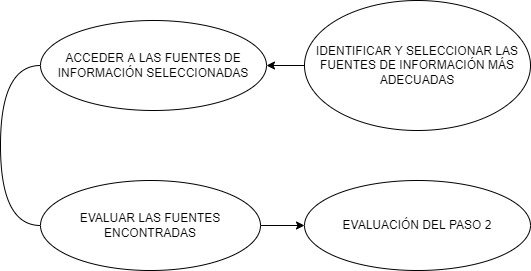
\includegraphics[width=0.70\textwidth]{Cap2/Figuras/Búsqueda y evaluación de información.jpg}
  \caption{Búsqueda y evaluación de fuentes de información. González (2007)}
  \label{fig:24}
\end{figure}

%------------------------------------------------------------
%	Subpaso 2a: Identificar y seleccionar las fuentes de información más adecuadas
%------------------------------------------------------------

\subsubsection{Subpaso 2a: Identificar y seleccionar las fuentes de información más adecuadas}
\label{secPaso2aCap2}

El objetivo de este subpaso es desarrollar la habilidad de reconocer las fuentes de información más adecuadas para la investigación, es decir, los recursos utilizados para extraer información. Existen diferentes fuentes de información, por lo que es importante la identificación de las fuentes de información que son de mayor utilidad para el proceso de investigación, dependiendo de las necesidades identificadas en el análisis de la definición y del problema de investigación.

Algunas fuentes de información más utilizadas son libros, blogs, páginas de internet, revistas, periódicos, videos, podcast, entre otros. Cada una de ellas cuenta con características que pueden aportar mayor o menor utilidad a la investigación, dependiendo del tema y la organización planeada en el paso de definición y planeación.

% REFERENCIA
Polo (2022) señala que existen tres diferentes tipos de fuentes de información:

\begin{itemize}
  \item \textbf{Fuentes primarias.} Las fuentes de información primarias son aquellas que son publicadas directamente por su autor por primera vez, y por tanto, es información que no ha sido filtrada, interpretada o evaluada previamente por un tercero. Tales como libros, notas de revista, notas periodísticas, reportes de investigación, fotografías, videos u obras de arte originales.Las fuentes de información primarias son aquellas que son publicadas directamente por su autor por primera vez, y por tanto, es información que no ha sido filtrada, interpretada o evaluada previamente por un tercero. Tales como libros, notas de revista, notas periodísticas, reportes de investigación, fotografías, videos u obras de arte originales.
  \item \textbf{Fuentes secundarias.} Las fuentes secundarias ofrecen información que ya ha sido procesada a partir de fuentes primarias en un orden específico. Es decir, proporciona información que aplica cierto criterio para dar a conocer información específica, tales como resúmenes, catálogos, diccionarios, enciclopedias, fuentes biográficas, bibliografías, atlas, manuales, entre otras.
  \item \textbf{Fuentes terciarias.} Estas fuentes funcionan como apoyo o guía, para encontrar información en fuentes primarias y secundarias. Tales como un índice de artículos generales de publicaciones de periódico, el catálogo de una biblioteca, una bibliografía, o el motor de búsqueda de un navegador web.
\end{itemize}

Entender las diferencias entre fuentes de información y sus características, aportan una habilidad para reconocer cuáles son las más adecuadas para la investigación, dependiendo del tema que se necesita investigar. Además, dominar la selección de tipos de fuentes de información, ayuda al estudiante a saber qué tan alejada está la información de hechos fidedignos, logrando con ello, conseguir información de mayor calidad, confiable y con mayores aportaciones al contenido de la investigación.

% REFERENCIA
Existen diferentes tipos de información que son importantes conocer, para enfocar de mejor forma las fuentes de información a utilizar. Burkhardt, MacDonald y Rathemacher (2003) señalan que existen cuatro tipos de información presentados a continuación:

\begin{itemize}
  \item \textbf{Información factual.} Es aquella información que tiene forma de comprobarse y que está basada en hechos. Este tipo de información no cambia y en todas las fuentes de información que se consulte, esta tiene exactamente los mismos datos. Tal es el caso de teorías físicas, matemáticas, métodos científicos probados, etc.
  \item \textbf{Información analítica.} Este tipo de información es el resultado de la interpretación y el análisis de la información factual. Es decir, es información resultante de la investigación de expertos en un tema y que por lo general se publica en libros o notas periodísticas. Esta información implica un proceso o reflexión de cómo se llegan a los resultados propuestos en la conclusión de la información.
  \item \textbf{Información subjetiva.} Esta información es resultado de la opinión y el punto de vista de un grupo o de un individuo sobre algún tema. Es información que contiene la perspectiva del autor o autores, sin ser necesariamente información fidedigna.
  \item \textbf{Información objetiva.} Es información que contiene la simplificación de un tema, del cual se toman diferentes fuentes de información para crear una síntesis de aspectos relevantes para un enfoque específico. Este tipo de información puede tener en su contenido una combinación de los diferentes tipos de información anteriores. Sin embargo, a diferencia de la información subjetiva, esta no incluye posturas de los autores.
\end{itemize}

La identificación de fuentes de información, así como el tipo de información que se requiere buscar para la investigación, son aspectos fundamentales que facilitan la búsqueda y la evaluación de fuentes, tomando en cuenta el origen de la información. A pesar de que varias de las fuentes de información pueden encontrarse en formato digital, es importante mencionar que cada fuente tiene características individuales que pueden sobresalir para realizar una mejor investigación de un tema específico.

Retomando el ejemplo, ¿crees que eres malo para las matemáticas?, la información relacionada con la pregunta puede surgir de un estudio psicológico o algún artículo matemático. Las fuentes de información más adecuadas para encontrar esta información pueden basarse en un estudio cognitivo o estadístico, sin importar si está publicado en internet o en un libro.

%------------------------------------------------------------
%	Subpaso 2b: Acceder a las fuentes de información seleccionadas
%------------------------------------------------------------

\subsubsection{Subpaso 2b: Acceder a las fuentes de información seleccionadas}
\label{secPaso2bCap2}

En este subpaso se utilizan diferentes estrategias para explorar las distintas fuentes de información de forma correcta.

Dependiendo del tipo de fuente de información, la forma en que se accede a esta varía. Cada fuente de información cuenta con una estrategia de búsqueda distinta, un índice para los libros, categorías o secciones para los periódicos, clases o motores de búsqueda para fuentes en la Internet, catálogos y códigos para una biblioteca, entre otros.

Es importante utilizar palabras clave en esta etapa para facilitar la búsqueda. Las palabras clave son términos sobresalientes del tema a investigar, que limita y facilita la búsqueda de la información. Es útil identificar estas palabras para realizar una búsqueda más rápida y precisa en las diferentes fuentes de información.

Además de identificar palabras clave, es primordial determinar cuáles son los aspectos involucrados en la búsqueda, con el fin de formular una frase que limite el tema dentro de la fuente de información. Es decir, se determinan aspectos como fechas, hechos importantes, teorías, personajes históricos, etc., para formar una frase a partir del aspecto a conocer y las palabras clave identificadas.

Una estrategia para poder formular estas frases, es tomar información del conjunto de preguntas secundarias de las cuales se pueden extraer aspectos específicos por conocer. Las palabras clave, en cambio, pueden obtenerse tanto de las preguntas secundarias como de la pregunta inicial, definida en el primer paso del Modelo Gavilán.

En esta etapa se consigue la ubicación de la información que puede ser relevante para la investigación o que puede contener datos que son indispensables para responder las preguntas secundarias. Todos estos resultados se almacenan en una bitácora para poder consultarlo posteriormente. Dependiendo del tipo de fuente de información, la bitácora debe almacenar información específica, como la URL para las páginas web, el número de la página de un libro, el artículo de una revista, la página de una enciclopedia, etc.

Cabe mencionar que es posible tener más de una fuente de información para cada una de las frases propuestas para la búsqueda. Puede ser una combinación de fuentes de información o una misma fuente de información de diferente autor.

Por ejemplo, algunas frases para encontrar información útil para la investigación, considerado la pregunta inicial y las preguntas secundarias son las siguientes:

\begin{itemize}
  \item Significado del trauma matemático.
  \item Autor del trauma matemático.
  \item Causas del trauma matemático.
  \item Solución al trauma matemático.
\end{itemize}

Las frases anteriores, son un apoyo para poder encontrar información de forma más relevante para la investigación. Los resultados de la búsqueda se pueden almacenar en una bitácora como en la Tabla \ref{tab:t3}.

\begin{table}[H]
  \begin{center}
    \begin{tabular}{ | p{2cm} | p{6cm} | p{2cm} | p{6cm} | }
      \hline
      No. DE FUENTE & INFORMACIÓN & FUENTE DE INFORMACIÓN & UBICACIÓN DE LA INFORMACIÓN \\ \hline
      1 & 
      \begin{itemize}
        \item Significado del trauma matemático
        \item Autor del trauma matemático
        \item Causas del trauma matemático
      \end{itemize} & Internet & \url{https://theconversation.com/crees-que-eres-malo-para-las-matematicas-puedes-sufrir-un-trauma-matematico-143507#:~:text=El%20'trauma%20matem%C3%A1tico'%20se%20manifiesta,las%20opciones%20escolares%20y%20 profesionales}
       \\ \hline

      2 & 
      \begin{itemize}
        \item Causas del trauma matemático
      \end{itemize} & Artículo digital & Novelo, S., Herrera, S., Díaz, J., Salinas, H. (2025), Temor a las matemáticas: causa y efecto
       \\ \hline
      
      3 & 
      \begin{itemize}
        \item Causas del trauma matemático
      \end{itemize} & Internet & \url{https://www.trahtemberg.com/articulos/3472-el-trauma-matematico.html}
       \\ \hline
      
      4 & 
      \begin{itemize}
        \item Solución al trauma matemático
      \end{itemize} & Internet & \url{https://harmonia.la/mente-y-emociones/salud-mental/te-consideras-malo-para-las-matematicas-quiza-sufriste-un-trauma}
       \\ \hline

    \end{tabular}
    \caption{Ejemplo de estrategias del subpaso 2b del Modelo Gavilán.}
    \label{tab:t3}
  \end{center}
\end{table}

%------------------------------------------------------------
%	Subpaso 2c: Evaluar las fuentes de información encontradas
%------------------------------------------------------------

\subsubsection{Subpaso 2c: Evaluar las fuentes de información encontradas}
\label{secPaso2cCap2}

Este subpaso tiene como objetivo desarrollar la habilidad de identificar cuáles son aquellas fuentes de información que son útiles para la investigación a partir de una evaluación considerando ciertos criterios de calidad para obtener los mejores resultados.

En Internet existe una cantidad inmensa de información sobre casi cualquier tema, sin embargo, no toda la información cuenta con las características de calidad que convierten el recurso en una buena fuente de información, ya que puede ser información errónea, poco clara e incluso sin sustentos. Es por ello que es necesario definir un criterio de calidad para determinar cuáles fuentes de información cumplen con las características necesarias para indagar y extraer información.

% REFERENCIA
González (2007), señala que algunos de los criterios que se pueden tomar en consideración para medir la calidad de una fuente de información son los siguientes:

\begin{itemize}
  \item Examinar el propósito de la fuente de información. Es decir, determinar brevemente el propósito para el cual fue creado el material, tal como propósitos de venta, informativo, científico, etc.
  \item Analizar los datos sobre el autor que escribió el contenido de la fuente de información. Es importante conocer información sobre su formación para determinar si domina el conocimiento en el área.
  \item Precisar la confiabilidad de la fuente de información a partir de los dos puntos anteriores.
\end{itemize}

Para el desarrollo de las habilidades de este subpaso, se puede generar una bitácora con todas las fuentes de información propuestas, así como los criterios de evaluación de calidad. La meta es determinar por cada una de ellas, cuáles son las fuentes que mejor cumplen con los criterios elegidos para ser una buena fuente de información. Estos pueden variar dependiendo del tipo de investigación que se quiere obtener como resultado.

Una vez identificados los criterios que se cumplen y los que no se cumplen, se procede a hacer un filtro de fuentes en los que se quedan aquellas que son más aptas y viables para encontrar la información que interesa para la investigación. Esta tarea ayuda a identificar y saber seleccionar de forma crítica cuáles son las fuentes que son más relevantes y que pueden aportar más, incluso sin haber leído el contenido aún.

Esta bitácora apoya a su vez a considerar las razones por las que una fuente de información es buena, regular o mala para la investigación, así como comprar sus características para desarrollar la habilidad de identificación de buenas fuentes de información.

Retomando las fuentes de información seleccionadas en el subpaso 2c, analizamos si la fuente de información es confiable para la investigación, tomando en cuenta los factores para medir la calidad de las fuentes, mencionado anteriormente, tal como se muestra en la Tabla \ref{tab:t4}

\begin{table}[H]
  \begin{center}
    \begin{tabular}{ | p{2cm} | p{4cm} | p{4cm} | p{6cm} | }
      \hline
      No. DE FUENTE & PROPÓSITO DE LA FUENTE & DATOS DEL AUTOR & CONFIABILIDAD DE LA FUENTE \\ \hline
      1 & Informativo, académico & Jennifer Ruef, profesor asistente de la Universidad de Oregon & Dado que el propósito de la fuente es informativo y el autor parece tener dominio sobre el tema, se concluye que esta fuente de información puede aportar información útil a la investigación. \\ \hline
      2 & Académico, investigación & Estudiantes y profesores de la Universidad Autónoma del Carmen & El propósito del artículo es bueno para fines de la investigación de ejemplo. Los autores parecen dominar los temas respecto a educación. \\ \hline
      3 & Académico, informativo & León Trahtemberg, Ingeniero Mecánico  con estudios en posgrado en Administración de la Educación & El propósito del artículo es bueno para fines de la investigación de ejemplo. Los autores parecen dominar los temas respecto a educación. \\ \hline
      4 & Informativo & Sin información del autor & En este caso, al no contar con información suficiente sobre la información del autor, puede surgir duda sobre la veracidad de la información, por lo que esta fuente de información podría omitirse o sustituirse por otra fuente que sea de calidad. \\ \hline

    \end{tabular}
    \caption{Ejemplo de estrategias del subpaso 2c del Modelo Gavilán.}
    \label{tab:t4}
  \end{center}
\end{table}

%------------------------------------------------------------
%	Subpaso 2d: Evaluación del paso 2
%------------------------------------------------------------

\subsubsection{Subpaso 2d: Evaluación del paso 2}
\label{secPaso2dCap2}

El objetivo de este subpaso es determinar si los subpasos anteriores lograron desarrollar de manera exitosa la habilidad de búsqueda y evaluación de información, dividido en cada una de sus etapas. Se determina si se obtuvieron los principios fundamentales para desarrollar criterios de calidad de selección de fuentes de información, basados en el objetivo de la fuente, el autor del contenido y la fiabilidad de la información, tomando como apoyo una bitácora con la comparación de cada fuente de información.

La evaluación de este paso es supervisada por un tutor a cargo del estudiante, para determinar con criterios independientes si se desarrollaron las habilidades para obtener fuentes de información que cumplan con los estándares planteados en los objetivos del segundo paso del Modelo Gavilán. Además, el supervisor brinda apoyo, observaciones y recomendaciones al investigador de cómo mejorar el proceso de investigación de fuentes y recursos.

Para tener una guía de cómo evaluar el desempeño del investigador, se proporciona una serie de preguntas divididas en cada uno de los subpasos del Modelo Gavilán con una medición en escala de cero a cinco. El equipo de EDUTEKA desarrolló algunas preguntas para el apoyo de la evaluación del segundo paso del Modelo Gavilán, llamado LISTA DE VERIFICACIÓN - EVALUACIÓN PASO 2 (MODELO GAVILÁN), que puede consultarse en EDUTEKA (2007).

%------------------------------------------------------------
%	Análisis de la información
%------------------------------------------------------------

\subsection{Análisis de la información}
\label{secPaso3Cap2}

El objetivo general de este paso es desarrollar las estrategias para determinar de forma crítica si la información seleccionada es útil, de calidad, relevante, confiable y aporta valor útil a la investigación. Este es uno de los pasos más complicados, ya que por lo general, a los estudiantes se les dificulta identificar información importante en textos demasiado extensos, así como comprender el contenido de la información de un tema completamente nuevo, por lo que es muy frecuente encontrar reportes de estudiantes basados en lo que se conoce como copy-paste (copiar y pegar la información sin analizarla).

El tercer paso del Modelo Gavilán se divide en tres subpasos que brindan herramientas para analizar la información, poniendo especial atención en diferentes aspectos de análisis y criterios de calidad, y la evaluación general del paso. Los subpasos mencionados anteriormente son los siguientes.

\begin{itemize}
  \item [3a] Elegir la información más adecuada para responder las preguntas secundarias.
  \item [3b] Leer, entender, comparar, y evaluar la información seleccionada.
  \item [3c] Responder las preguntas secundarias.
  \item [3d] Evaluación del paso 3.
\end{itemize}

El primer subpaso consiste en leer la información contenida en las fuentes de información, tratando de comprender y asociar la información con datos que ya se conocen sobre el tema. Además, el estudiante procesa la información de cada una de las fuentes, para dar respuesta al conjunto de preguntas secundarias, separando los párrafos u oraciones que contienen la respuesta para cada pregunta secundaria.

La segunda fase de los subpasos, consiste en hacer un análisis de la información de cada una de las diferentes frases u oraciones extraídas, comparando los resultados de un recurso con otro, con el fin de confirmar datos, complementar información, determinar cuál contiene mayor valor para la respuesta a cada pregunta secundaria o incluso distinguir si dos fuentes de información se contradicen.

Posteriormente, se procede a realizar un proceso de comprensión de información, en la que el estudiante da respuesta a cada una de las preguntas secundarias a partir de la información que analizó de las fuentes de información. Esta respuesta no está basada en las palabras del autor de las fuentes de información sino que se expresa en las propias palabras del estudiante, con base en los datos de cada recurso analizado.

Estos subpasos mencionados a grandes rasgos, se pueden apreciar en el orden en que son efectuados en la Figura \ref{fig:25}.

\begin{figure}[H]
% \begin{figure}
  \centering
  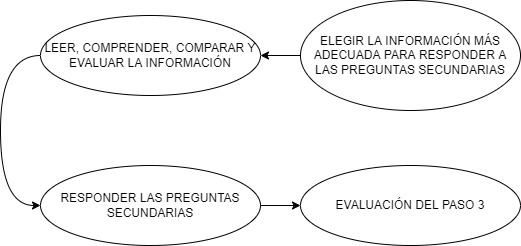
\includegraphics[width=0.70\textwidth]{Cap2/Figuras/Análisis de la información.jpg}
  \caption{Análisis de la información. González (2007)}
  \label{fig:25}
\end{figure}

%------------------------------------------------------------
%	Subpaso 3a: Elegir la información más adecuada para responder las preguntas secundarias
%------------------------------------------------------------

\subsubsection{Subpaso 3a: Elegir la información más adecuada para responder las preguntas secundarias}
\label{secPaso3aCap2}

Como objetivo de este subpaso se tiene el desarrollar la habilidad de selección de información, que responda de mejor manera a las preguntas secundarias. Este subpaso conlleva a prestar especial atención a la información que realmente es útil, lo cual lo vuelve uno de los pasos más complejos del Modelo Gavilán.

Por lo general, cuando se realiza un proceso de copy-paste con una fuente de información, se analiza superficialmente cuál es la información que resuelve de mejor manera el problema de información. En este subpaso, se analiza la selección de párrafos y datos que responden de mejor manera a las preguntas secundarias, con la diferencia de que no se copia y se pega la información, sino que se extrae sólo lo importante y relevante para la investigación.

% REFERENCIA
González (2007), señala que una estrategia para poder seleccionar de manera eficiente la información es considerar los siguientes puntos:

\begin{itemize}
  \item Determinar y preguntarse qué es lo que se requiere saber de la pregunta secundaria en cuestión. Es decir, identificar los fragmentos de información que dan respuesta a las preguntas.
  \item Reflexionar y seleccionar las respuestas que son más aptas para responder la pregunta secundaria y marcar o almacenar el fragmento correspondiente . Es importante que a la par de la selección de información, se incluya la referencia de dónde se obtuvieron dichos datos.
  \item Repetir el proceso con cada una de las preguntas secundarias, usando los fragmentos de información encontrados.
\end{itemize}

Retomando el ejemplo de investigación, se puede ver el ejemplo de la Tabla \ref{tab:t5}

\begin{table}[H]
  \begin{center}
    \begin{tabular}{ | p{2cm} | p{4cm} | p{7cm} | p{3cm} | }
      \hline
      EXTRACTO & PREGUNTA SECUNDARIA & RESPUESTA & REFERENCIA \\ \hline
      1 & ¿Qué es el trauma matemático? & Es la manifestación de miedo o temor por equivocarse, enfocado a contextos relacionados a matemáticas &
      Fuente 1
      \begin{itemize}
        \item Párrafo 5
      \end{itemize}
       \\ \hline

      2 & ¿Quien definió el significado de trauma matemático? & Definido en este artículo por Jennifer Ruef &
      Fuente 1
      \\ \hline
    
      3 & ¿Cuándo se definió el trauma matemático? & La investigación y la definición surgen a partir de la intriga del origen de la dificultad por aprender matemáticas &
      Fuente 1
      \begin{itemize}
        \item Párrafo 2
        \item Párrafo 3
      \end{itemize}
       \\ \hline

      4 & ¿Quienes pueden ser afectados por el trauma matemático? & El problema es que el alumno sigue reprobando matemáticas a pesar de ser una materia básica y sobre todo cotidiana; la razón de lo anterior se debe a que todos los días usamos las matemáticas. &
      Fuente 2
      \begin{itemize}
        \item Página 3
        \item Párrafo 1
      \end{itemize}
       \\ \hline

      5 & ¿Quienes pueden ser afectados por el trauma matemático? & Cuando las personas comparten sus historias conmigo, hay temas comunes. Estos incluyen a alguien diciéndoles que $"$no eran buenos en matemáticas$"$. Uno de los mayores desafíos a los que se enfrentan los educadores de matemáticas de Estados Unidos es ayudar a la gran cantidad de maestros de primaria que se enfrentan a un 'trauma matemático' &      
       Fuente 1
       \begin{itemize}
         \item Párrafo 2
         \item Párrafo 4
       \end{itemize}
        \\ \hline
      
      6 & ¿Cómo puede presentarse el trauma matemático? & pánico por las pruebas de matemáticas programadas, o quedando atrapado en algún tema de la materia y luchando para superarlo &
       Fuente 1
       \begin{itemize}
         \item Párrafo 2
       \end{itemize}
        \\ \hline
      
      7 & ¿Cómo puede presentarse el trauma matemático? & Esto hace que ellos se sientan desmotivados durante su proceso de aprendizaje, por lo que su conducta es de negación hacia las matemáticas al considerar poco probable la adquisición de los conocimientos. El fracaso, es el mayor factor por el cual las personas le tienen miedo a las matemáticas. El fracaso y el miedo dan mucho que decir al momento de pasar al pizarrón o sacar una nota no aprobatoria en el examen. Así mismo el rechazo de la sociedad puede afectar porque si el alumno no saca calificaciones aceptables &
       Fuente 2
       \begin{itemize}
         \item Página 2
         \item Página 5
         \item Página 10
       \end{itemize}
        \\ \hline

    \end{tabular}
  \end{center}
\end{table}

\begin{table}[H]
  \begin{center}
    \begin{tabular}{ | p{2cm} | p{4cm} | p{7cm} | p{3cm} | }
      \hline
      8 & ¿Cómo puede presentarse el trauma matemático? & Una de las razones de esta $"$ansiedad numérica$"$ tiene que ver con la forma en que se enseña la matemática, basada en la memorización y las fórmulas jeroglíficas, los tests matemáticos y la naturaleza blanco/negro de los problemas que solo admiten una respuesta correcta. Sacar malas notas en los exámenes resulta ser una bomba fulminante. &
        Fuente 3
        \begin{itemize}
          \item Párrafo 3
        \end{itemize}
         \\ \hline
      
      9 & ¿Qué tipo de ejercicios se pueden realizar para mejorar en matemáticas? & que hacen que las personas jueguen con números, como Sudoku, KenKen o ciertos juegos de cartas, crean una necesidad intelectual de usar datos matemáticos que ayudan a los niños a desarrollar la fluidez de los datos. Pedirles a los niños que expliquen su pensamiento, usando palabras, imágenes u objetos, valida la importancia de sus ideas. &
         Fuente 1
         \begin{itemize}
           \item Párrafo 12
         \end{itemize}
          \\ \hline

      10 & ¿Qué estrategias se pueden seguir para practicar ejercicios matemáticos? & Replantear los errores como exploraciones. No tener una respuesta correcta no significa que todo pensamiento sea incorrecto. Pedirles a los niños que expliquen su pensamiento también ayuda a comprender lo que saben ahora y lo que podrían aprender a continuación. Segundo, no hagas daño. Es importante que los padres eviten enviarles a los niños mensajes de que no son matemáticos. &
      
          Fuente 1
          \begin{itemize}
            \item Párrafo 13
            \item Párrafo 14
          \end{itemize}
           \\ \hline

    \end{tabular}
    \caption{Ejemplo de estrategias del subpaso 3a del Modelo Gavilán.}
    \label{tab:t5}
  \end{center}
\end{table}

%------------------------------------------------------------
%	Subpaso 3b: Leer, entender, comparar, y evaluar la información seleccionada
%------------------------------------------------------------

\subsubsection{Subpaso 3b: Leer, entender, comparar, y evaluar la información seleccionada}
\label{secPaso3bCap2}

El objetivo de este subpaso es desarrollar las habilidades para encontrar relaciones entre los fragmentos de información seleccionados, de tal forma que se pueda determinar, para cada una de las preguntas secundarias, qué información puede fungir como complemento, comparación, verificación, ejemplo, o dato extra.

Esta es una fase en la que se determinan relaciones entre la información seleccionada de los diferentes recursos para evaluar si es necesario profundizar en dicha fuente o si es necesario considerar otros aspectos del tema. En caso de ser necesario, se consideran otros aspectos o se profundiza en la fuente actual, pero también se puede recurrir a la consulta de más fuentes de información, mismas que se evalúan y seleccionan como en el paso dos del Modelo Gavilán, referente a la búsqueda y evaluación de fuentes.

Cabe resaltar que dados los posibles casos de profundización o ampliación de información, se debe retornar a pasos anteriores y repetir cada una de las fases del paso dos, hasta que se concrete la información suficiente y necesaria para tener como resultado una investigación completa, clara y con información de calidad.

En la Tabla \ref{tab:t6} se muestra un ejemplo de comparación y evaluación de los extractos obtenidos en el subpaso 3a.

\begin{table}[H]
  \begin{center}
    \begin{tabular}{ | p{4cm} | p{5cm} | p{7cm} | }
      \hline
      EXTRACCIONES & COMPARACIÓN & EVALUACIÓN \\ \hline
      1 y 2 & Complemento & Información relevante para la investigación, ya que proporciona una definición del trauma matemático y su autor. \\ \hline
      3 & Complementario a los extractos 1 y 2 & La información de cómo surge el trauma matemático no es relevante para la investigación, por lo que este se puede omitir. \\ \hline
      4 y 5 & Complemento & Información relevante para la investigación, que contiene los efectos del trauma matemático \\ \hline
      7 y 8 & Ejemplo & Información relevante de presentación de trauma matemático, así como ejemplos. \\ \hline
      9 y 10 & Ejemplo & Información relevante de cómo tratar el trauma matemático y ejemplos de ejercicios \\ \hline
    \end{tabular}
    \caption{Ejemplo de estrategias del subpaso 3b del Modelo Gavilán.}
    \label{tab:t6}
  \end{center}
\end{table}

%------------------------------------------------------------
%	Subpaso 3c: Responder las preguntas secundarias
%------------------------------------------------------------

\subsubsection{Subpaso 3c: Responder las preguntas secundarias}
\label{secPaso3cCap2}

El objetivo principal de este subpaso es desarrollar las estrategias para que el estudiante adquiera la habilidad para responder a cada una de las preguntas secundarias con sus propias palabras.

En este punto del Modelo Gavilán, el estudiante ya conoce las respuestas a cada una de las preguntas secundarias, así como posibles complementos, ejemplos e incluso diferentes puntos de vista. Esta información permite tener una idea del tema general, así como aspectos específicos que son relevantes para la investigación. Los fragmentos recabados sobre las respuestas a las preguntas y la información extra, faculta al estudiante para poder responder cada pregunta secundaria con sus propias palabras, así como desarrollar una aproximación a la estructura de la cada una de las respuestas.

Al responder las preguntas secundarias con palabras propias, se demuestra y se refleja un entendimiento del tema, así como un buen proceso de análisis de la información. Además se muestra el razonamiento que se realiza por parte del estudiante para manifestar el conocimiento aprendido durante este paso.

En la Tabla \ref{tab:t7} se muestra un ejemplo de posibles respuestas de estudiantes a cada una de las preguntas secundarias.

\begin{table}[H]
  \begin{center}
    \begin{tabular}{ | p{8cm} | p{8cm} | }
      \hline
      PREGUNTA SECUNDARIA & RESPUESTA CON PALABRAS DEL ESTUDIANTE \\ \hline
      ¿Qué es el trauma matemático? & Es la fobia o temor por equivocarse al resolver ejercicios matemáticos. \\ \hline
      ¿Quién definió el significado de trauma matemático? & La profesora Jennifer Ruef. \\ \hline
      ¿Cuándo se definió el trauma matemático? & Surgió a partir del cuestionamiento de porqué a algunos de los estudiantes se les complican las matemáticas. \\ \hline
      ¿Quiénes pueden ser afectados por el trauma matemático? & Todos en general, especialmente estudiantes y algunos profesores de matemáticas. \\ \hline
      ¿Cómo puede presentarse el trauma matemático? & Puede presentarse como miedo, rechazo por parte de compañeros y familiares. También puede presentarse como inseguridad de la capacidad de poder resolver problemas matemáticos, lo cual causa desmotivación por querer aprender. \\ \hline
      ¿Qué tipo de ejercicios se pueden realizar para mejorar en matemáticas? & Algunos juegos que desarrollen la habilidad matemática, tal como sudokus o cartas. \\ \hline
      ¿Qué estrategias se pueden seguir para practicar ejercicios matemáticos? & Una estrategia es reconocer  que no obtener la respuesta correcta a un problema, no es malo. Por el contrario, está bien equivocarse y aprender de los errores para no cometerlos en los próximos ejercicios. Otra estrategia es evitar decir a los estudiantes que son malos en matemáticas.
       \\ \hline
    \end{tabular}
    \caption{Ejemplo de estrategias del subpaso 3c del Modelo Gavilán.}
    \label{tab:t7}
  \end{center}
\end{table}

%------------------------------------------------------------
%	Subpaso 3d: Evaluación del paso 3
%------------------------------------------------------------

\subsubsection{Subpaso 3d: Evaluación del paso 3}
\label{secPaso3dCap2}

Este paso de evaluación le concierne al tutor a cargo de la valoración de la investigación realizada por el estudiante. En esta evaluación se mide el desarrollo de las habilidades para analizar información a partir de la comprensión, el análisis, la relación y comparación de la información.

Se determina si se cumplieron los objetivos de cada subpaso y se logró el resultado esperado, para dar respuesta correcta y de calidad con palabras propias a las preguntas secundarias, con base en la atención y análisis de las relaciones que existieron entre diferentes fragmentos de información para una sola pregunta.

Los criterios a considerar para la evaluación del análisis de información pueden variar y pueden ser ajustados por el tutor de la investigación. El equipo de EDUTEKA desarrolló una lista de verificación que puede fungir como guía para determinar qué tan bien se lograron los objetivos de los subpasos del tercer paso del Modelo Gavilán, que puede consultarse en EDUTEKA (2007).

%------------------------------------------------------------
%	Síntesis y socialización de la información
%------------------------------------------------------------

\subsection{Síntesis y socialización de la información}
\label{secPaso4Cap2}

El objetivo de este último paso del Modelo Gavilán, es desarrollar las estrategias para que el estudiante pueda adquirir las habilidades necesarias para sintetizar y organizar la información de forma clara y enfocada en el resultado de la investigación.

En esta etapa se busca resolver el problema de investigación a los que se enfrentan los estudiantes al momento de comenzar la búsqueda de información. Para lograr este resultado, se recaba todo el esfuerzo y resultados obtenidos en los pasos anteriores, de tal forma que se pueda estructurar para resolver cada aspecto considerado en las preguntas secundarias y, en conjunto, la pregunta inicial.

Además, se busca que toda la información recopilada, que ya cuenta con cierta estructura, se pueda expresar o representar por el medio de comunicación adecuado, para que la investigación pueda ser entendida por un tercero.

Los subpasos del cuarto y último paso del Modelo Gavilán expresan cada una de las acciones y tareas para desarrollar las habilidades de síntesis y socialización de información. Los pasos del cuarto paso del Modelo Gavilán son los siguientes.

\begin{itemize}
  \item [4a.] Responder la pregunta inicial
  \item [4b.] Elaborar un producto concreto
  \item [4c.] Comunicar los resultados de la investigación
  \item [4d.] Evaluación del paso 4 y el proceso
\end{itemize}

Estos subpasos se siguen como en la Figura \ref{fig:26}.

\begin{figure}[H]
% \begin{figure}
  \centering
  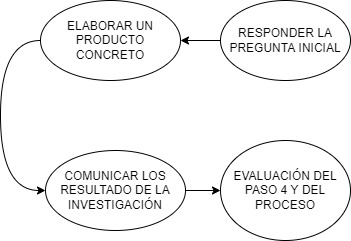
\includegraphics[width=0.60\textwidth]{Cap2/Figuras/Síntesis y socialización de información.jpg}
  \caption{Síntesis y socialización de la información. González (2007)}
  \label{fig:26}
\end{figure}

%------------------------------------------------------------
%	Subpaso 4a: Responder la pregunta inicia
%------------------------------------------------------------

\subsubsection{Subpaso 4a: Responder la pregunta inicia}
\label{secPaso4aCap2}

El objetivo de este subpaso consta de adquirir las habilidades para poder recuperar y relacionar información, para dar respuesta completa a la pregunta inicial del problema de investigación.

Este paso requiere de un análisis profundo para identificar distintos aspectos del problema general y relacionarlos entre sí, para construir una respuesta completa que sea clara, coherente y aporte la información requerida por los criterios de la investigación. Es un proceso de unificación, que surge a partir de las respuestas de las preguntas secundarias para crear un texto que cubra todos los detalles solicitados de un tema, así como aportaciones extras del estudiante.

% REFERENCIA
González (2007), propone una estrategia para organizar la información y conocer los diferentes puntos de un tema. Esta estrategia consiste en elaborar mapas que permitan distribuir y organizar la información en diferentes categorías, tal como un mapa conceptual u otra representación de información. Estas herramientas clarifican la forma en que se distribuye la información y se representa de forma gráfica.

Al construir la representación general con cada fragmento de datos obtenidos en el tercer paso del Modelo Gavilán, se sintetiza la información como una sola para dar una respuesta completa a la pregunta inicial, considerando todos los componentes que apoyan a sostener la investigación obtenida. En consecuencia de la elaboración de esta representación gráfica, se produce un criterio para unificar la información en una sola respuesta completa a la pregunta inicial, así como para encontrar datos faltantes o categorías que podrían complementar la información final.

A continuación se muestra un esquema donde se distribuye la información obtenida en el subpaso 3c del ejemplo  desarrollado en el paso anterior, en la Figura \ref{fig:27}.

\begin{figure}[H]
% \begin{figure}
  \centering
  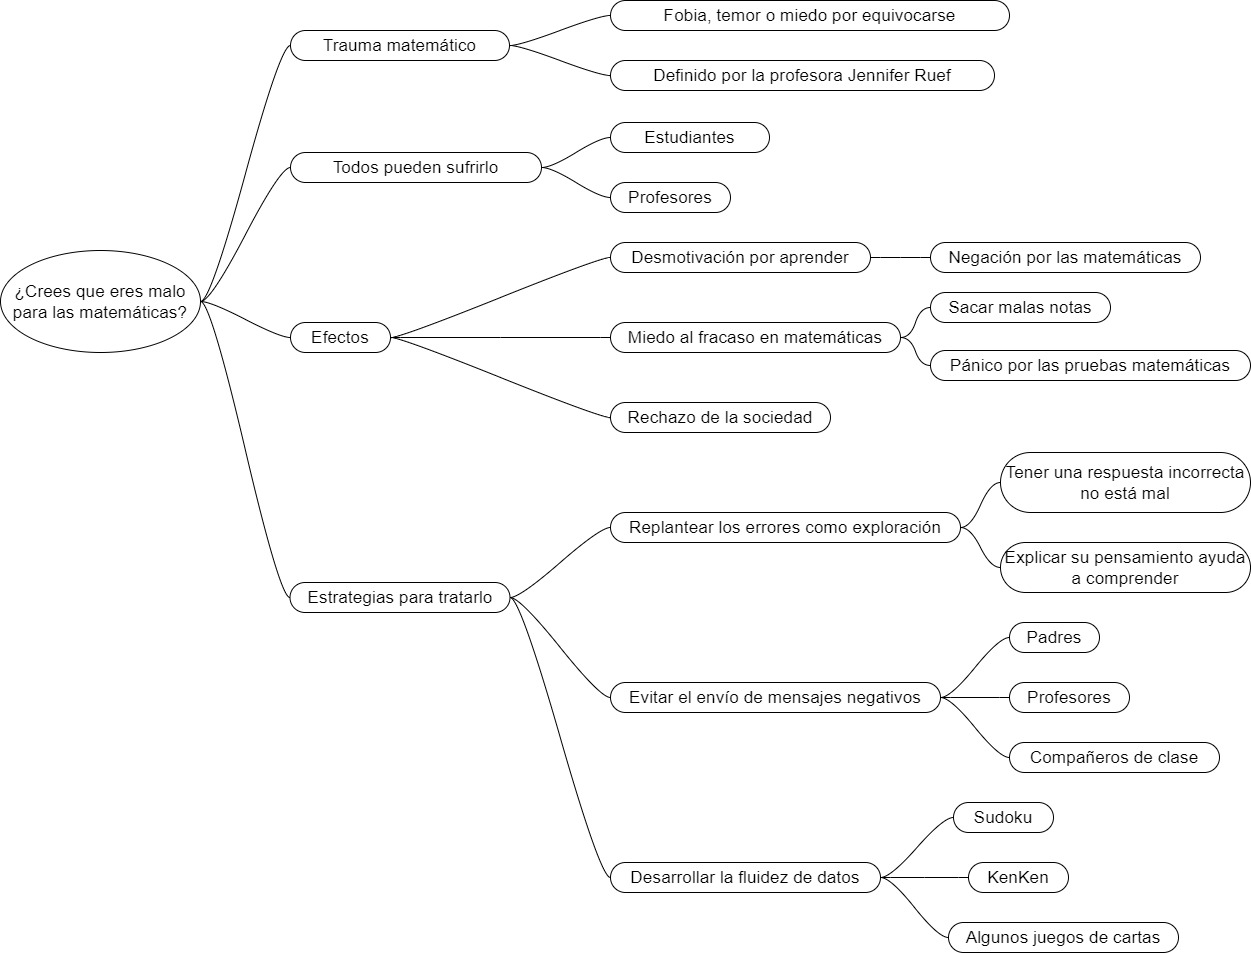
\includegraphics[width=0.70\textwidth]{Cap2/Figuras/Ejemplo de estraregia del subpaso 4a.jpg}
  \caption{Ejemplo de estrategias del subpaso 4a del Modelo Gavilán.}
  \label{fig:27}
\end{figure}

%------------------------------------------------------------
%	Subpaso 4b: Elaborar un producto concreto
%------------------------------------------------------------

\subsubsection{Subpaso 4b: Elaborar un producto concreto}
\label{secPaso4bCap2}

El objetivo de este subpaso es llevar la información recopilada a un producto que cuente con todos los datos necesarios que respondan a la pregunta inicial en forma de ensayo, artículo, mapa conceptual, dibujo, de esquema, video, entre otros.

En esta etapa del cuarto paso, es necesario definir una forma de representar la información, misma que puede estar estipulada por un tutor o en su defecto, ser elegida por el estudiante, considerando la opción más viable para expresar los resultados. Es importante a su vez, asegurar que la información que ya se analizó y organizó, haya sido entendida por el estudiante, con el fin de adquirir los conocimientos esperados en la investigación del tema.

Es valioso mencionar que la información, dependiendo de sus características, se acopla más a un esquema de representación que a otro, por lo que el estudiante puede utilizar diferentes esquemas de representación en el producto final. Es decir, pueden existir combinaciones como mapas en un ensayo, gráficas en un artículo, imágenes en mapas conceptuales, etc.

Por otro lado, dependiendo del tipo de entrega o investigación, esta puede ser construida de forma digital, como una presentación, un video, una imagen, etc., así como de forma física como un dibujo, un ensayo, una tarjeta, etc. Este punto también se encuentra determinado por la elección de un tutor o del estudiante.

Para la elección de estos aspectos, es considerablemente necesario conocer las características con las que cuenta cada esquema de representación de información, para explotar así sus ventajas.

Finalmente, se pone en consideración la forma en que el estudiante adquirió el dominio y comprensión del tema de investigación, ya que no sólo es importante aprender a poner en práctica y adquirir las habilidades del modelo gavilán, sino también aprender contenido útil sobre el tema involucrado en la investigación, de tal forma que se expanda el conocimiento del tema comparado con lo que se conocía antes de la investigación.

Retomando el ejemplo con la información del subpaso anterior, se presenta a continuación un breve reporte en la Tabla \ref{tab:t8}.

\begin{table}[H]
  \begin{center}
    \begin{tabular}{ | p{16cm} | }
      \hline
      RESULTADO FINAL DE LA INVESTIGACIÓN - REPORTE \\ \hline
      ¿Crees que eres malo para las matemáticas? Esto puede ser causa de un trauma matemático. El trauma matemático, definido por la profesora Jennifer Ruef, es el miedo, fobia o temor por equivocarse en ejercicios o la resolución de problemas matemáticos.
      
      El trauma matemático se presenta principalmente en estudiantes y profesores, sin embargo, cualquier persona puede presentar un trauma matemático, provocando desmotivación por el aprendizaje, miedo al fracaso o rechazo por la sociedad. Esto puede causar que el afectado desarrolle una negación por las matemáticas, obtener malas calificaciones o incluso generar pánico en pruebas matemáticas.
      
      Para prevenir y evitar el trauma matemático, se pueden tomar en cuenta los siguientes aspectos:

      \begin{itemize}
        \item Replantear los errores como exploración. Es importante trabajar en la aceptación y la determinación para saber que una respuesta incorrecta en las pruebas de matemáticas no está mal. Por el contrario, se puede explorar y explicar lo que el alumno piensa para comprender mejor los temas, con el fin de aprender de los errores, de tal forma que en una prueba siguiente, ya se tendrá conocimiento para no cometer el mismo error.
        \item Evitar el envío de mensajes negativos. Algunas personas piensan que son malas en matemáticas porque así lo dijo un profesor, algún compañero de clase o incluso los padres. Es importante evitar los comentarios negativos, para no generar angustia y provocar un trauma matemático.
        \item Desarrollar actividades donde se trabaja la fluidez de datos. Para poner en desarrollo y práctica la habilidad matemática, se recomienda realizar actividades donde intervenga el análisis matemático y el proceso de datos, tal como el sudoku, KenKen o algunos juegos de cartas.
      \end{itemize}

      \\ \hline
    \end{tabular}
    \caption{Ejemplo de estrategias del subpaso 4c del Modelo Gavilán.}
    \label{tab:t8}
  \end{center}
\end{table}

%------------------------------------------------------------
%	Subpaso 4c: Comunicar los resultados de la investigación
%------------------------------------------------------------

\subsubsection{Subpaso 4c: Comunicar los resultados de la investigación}
\label{secPaso4cCap2}

En este paso se desarrollan las habilidades para poder expresar la información que se obtuvo en el esquema del subpaso anterior de forma oral, de tal manera que se pueda comunicar como exposición hacia un tutor o un grupo de personas.

Las actividades de este subpaso involucran varios aspectos que pueden manifestar el buen trabajo realizado en los pasos del Modelo Gavilán. Tales como hablar con buen dominio sobre el tema, tener cierta organización en la forma en que se expresan las ideas del tema, conocer datos específicos de un tema general, exponer ejemplos que clarifiquen un tema y finalmente, tener la habilidad de responder todas las dudas o cuestiones que surjan al final de una exposición.

A pesar de tener un documento con toda la información necesaria para responder la pregunta inicial vinculada a un tema, es importante mencionar que en una exposición no todos los datos son relevantes o no es necesario profundizar tanto en ellos, ya que la investigación del esquema del subpaso anterior puede ser muy amplio.

Es primordial recalcar que en una exposición, se tiene por objetivo la comunicación del tema y el tipo de audiencia al que se dirige el conocimiento. González (2007) señala que algunos puntos importantes a considerar en este subpaso son los siguientes.

\begin{itemize}
  \item Comunicar las ideas más generales de forma clara y comprensible para la audiencia.
  \item Generar recursos gráficos que sirvan de apoyo visual para dar un mejor resultado al entendimiento de información.
  \item El uso correcto y claro de ejemplos y analogías con los que la audiencia pueda sentirse identificada para entender el tema.
  \item Considerar, sin excepción, el respeto a los derechos de autor de los recursos de donde se extrae la información.
\end{itemize}

%------------------------------------------------------------
%	Subpaso 4d: Evaluación del paso 4 y el proceso
%------------------------------------------------------------

\subsubsection{Subpaso 4d: Evaluación del paso 4 y el proceso}
\label{secPaso4dCap2}

El objetivo de este último subpaso consiste en evaluar las habilidades obtenidas para poder sintetizar y organizar la información. Además, al ser el último paso del Modelo Gavilán, también se incluye la evaluación del resultado logrado a partir de todo el proceso desde el primer paso hasta este punto.

Tal como en la evaluación de los pasos anteriores, el tutor del estudiante es el encargado de determinar y medir si los objetivos esperados de cada subpaso se concluyeron de forma satisfactoria. Así mismo, el tutor tiene el cargo de evaluar los resultados finales de todo el proceso hecho, siguiendo los pasos del Modelo Gavilán.

Para determinar si los objetivos se cumplieron, se establecen criterios de evaluación establecidos por el mismo tutor, donde se destacan aspectos importantes como un correcto análisis para la síntesis, una buena organización, buen dominio del tema para exposición, la capacidad de comunicar ideas críticas de un tema, entre otros. Algunos aspectos propuestos por el equipo de EDUTEKA, llamado LISTA DE VERIFICACIÓN - EVALUACIÓN PASO 4 (MODELO GAVILÁN), que pueden ser considerados para la evaluación, pueden encontrarse en EDUTEKA (2007). 

Cabe mencionar que los criterios de evaluación establecidos en la lista son un apoyo para la evaluación. El tutor de la investigación puede agregar u omitir criterios a evaluar.

%------------------------------------------------------------
%	Resumen
%------------------------------------------------------------

\section{Resumen}
\label{secResumenCap2}

En este capítulo se define la competencia de manejo de información, como un conjunto de habilidades, conocimientos y actitudes que un estudiante requiere para contextualizar y saber de manera precisa los detalles que se requieren extraer para un tema, así como desarrollar estrategias de búsqueda de la información más apta para utilizar como resultado de una investigación final. Por otra parte, la CMI también tiene el objetivo de desarrollar habilidades para obtener la capacidad de crear preguntas específicas y aplicarlas para concretar o detallar la información filtrada de las mejores fuentes de información.

A su vez, se menciona que una competencia se compone de dos factores: capacidades y actitudes. Por un lado, las capacidades se dividen en otras dos partes: conocimientos, que es todo aquello que se sabe sobre un tema; y las habilidades, que corresponde a la capacidad de usar la información que se sabe para resolver algún problema. Por otra parte, las actitudes se refieren a la buena disposición de lograr un objetivo.

Entre las metodologías para el desarrollo de la CMI, se encuentra la metodología conocida como El Modelo Gavilán, la cual es una metodología que se basa en cuatro pasos principales.

\begin{enumerate}
  \item Definición del problema de investigación.
  \item Búsqueda y evaluación de la información.
  \item Análisis de la información.
  \item Síntesis de la información.
\end{enumerate}

A su vez, cada uno de los pasos mencionados anteriormente, se dividen en subpasos, que proponen el desarrollo de habilidades específicas para poner cumplir los objetivos planteados en la CMI.

Para el desarrollo del proyecto, se toma como referencia el Modelo Gavilán para la construcción de la skill. Los autores del Modelo Gavilán mencionan que las habilidades desarrolladas en cada subpaso fungen como una propuesta para su aplicación, sin embargo, estas pueden ser adaptadas para el funcionamiento más adecuado de la metodología. Es importante mencionar que se considera una adaptación de algunos subpasos del Modelo Gavilán. La adaptación del Modelo Gavilán a la skill será descrita en el capítulo 4.
